\section{Zielsetzung}
\label{Zielsetzung}
Ziel dieses Versuches ist es die Wellenlänge eines Lasers zu bestimmen unter Zuhilfenahme des Michelson-Interferometers.
Außerdem soll der Brechungsindex von Luft bestimmt werden.

\section{Theorie}
\label{sec:Theorie}
Im Interferometer treten Interferenzeffekte auf, weswegen im Folgendem die Vorraussetzungen für Interferenz vorgestellt werden.

\subsection{Interferenz und Kohärenz von Licht}
\label{Int&Ko_theo}

Licht wird als elektromagnetische Welle angenommen und seine Ausbreitung kann mit den Maxwellgleichungen beschrieben werden.
Die Beschreibung der Lichtwelle erfolgt über die Feldstärke
\begin{equation}
    \vec{E}(x,t) = \vec{E_0} \cos(kx-wt-\delta),
    \label{eqn:Licht}
\end{equation}
wobei $x$ die Ortskoordinate, $k$ die Wellenzahl ist, welche den Zusammenhang $k = \frac{2\pi}{\lambda}$ mit der Wellenlänge $\lambda$ besitzt. 
$w$ ist die Kreisfrequenz und $\delta$ ist der Phasenwinkel.
Die Intensität $I$ des Lichtes die messbare Größe, welche durch $I = const \lvert \vec{E} \rvert^2$ berechnet werden kann.
Sie gibt den Zeitmittelwert der Lichtleistung an, die auf eine Flächeneinheit trifft. 
Wenn zwei Lichtwellen auf einem Punkt zusammentreffen, überlagern sie sich nach dem Suberpositionprinzip und für die Intensität gilt
\begin{equation*}
    I_{\text{ges}} = \frac{1}{t_2 - t_1} \int_{t_1}^{t_2} | \vec{E}(x,t)|^2 \, \symup{d}t  = \frac{1}{t_2 - t_1} \int_{t_1}^{t_2} | \vec{E_1}+ \vec{E_2}|^2 (x,t) \, \symup{d}t .
\end{equation*}
Der Beobachtungszeitraum sollte groß gegenüber der Periodendauer sein.\\
Beide Wellen besitzten die Form (\ref{eqn:Licht}), so ergibt sich die Gesamtintensität zu 
\begin{equation*}
    I_{\text{ges}} = 2\vec{E_0}^2(1+\text{cos}(\delta_2 - \delta_1)), 
\end{equation*}
wobei der Interferenzterm zeigt, dass sich die einzelnen Lichtwellen nicht einfach addieren.\\
\\
Eine wichtige Vorraussetzung für Interferenz ist kohärentes Licht, also dass die Parameter $k$, $w$ und $\delta$ in der 
\autoref{eqn:Licht} feste Werte besitzen.
Lichtquellen, die kohärentes Licht erzeugen, sind zum Beispiel Laser. 
Aber auch mit konventionellen Lichtquellen, kann mit einer Versuchsanordnung wie in \autoref{fig:Abb1} kohärentes Licht erzeugt werden.
\begin{figure}[H]
    \centering
    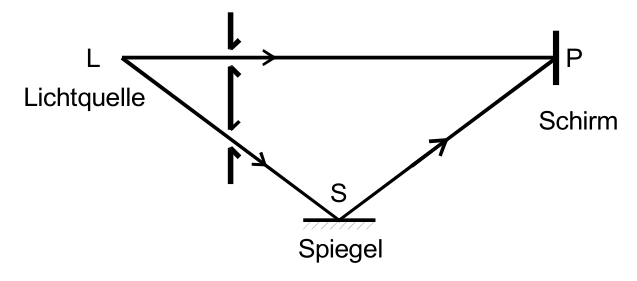
\includegraphics[width=0.3\textwidth]{build/Abb1.PNG}
    \caption {Prinzipielle Versuchsanordnung zur Erzeugung kohärentem Licht aus einer konventionellen Lichtquelle \cite[3]{V401}.}
    \label{fig:Abb1}
\end{figure}
Dazu wird das Licht aus einer Lichtquelle durch eine Doppelblende aufgeteilt, wobei ein Strahl auf direktem Weg auf einen Schirm trifft und
ein andere Strahl wird an einem Spiegel reflektiert und trifft auf den gleichen Auftreffpunkt auf.
Es ist zu beachten, dass der Emissionsakt nur eine endliche Zeit $\tau$ andauert, also besitzt der Wellenzug eine endliche Länge.
Wenn der Wegunterschied $\Delta$ (in \autoref{fig:Abb1} gilt $\Delta = \overline{\text{LSP}} - \overline{\text{LP}} $) deutllich größer ist 
als die Länge des Wellenzuges,treten keine Interferenzeffekte auf.
Der Grund dafür ist, dass die Lichtwellen, welche zeitgleich an de Punkt $P$ ankommen, keine feste Phasenbeziehung besitzen und somit nicht
mehr kohärent sind.
Der Wegunterschied, bei dem gerade keine Interferenzeffekte auftreten, wird Kohärenzlänge $\ell$ genannt.\\
Nach dem Fourierschem Theorem kann ein Wellenzug endlicher Länge nicht monochromatisch sein.
Jedoch ist polychromatisches oder nicht-monochromatisches Licht nicht interferenzfähig.
Deswegen muss das Frequenzspektrum so schmal oder der Wegunterschied so klein sein, dass die Maxima- und Minimabedingungen von zwei Wellenlängen
nicht an demselben Ort realisiert werden können.

\subsection{Prinzipieller Aufbau des Michelson-Interferometers}
\label{Aufbau_theo}
Das Michelson-Interferometer wurde entwickelt um im Michelson-Morley-Experiment den Äther nachzuweisen, was nicht funktioniert hat, jedoch werden 
ähnliche Interferometer dazu benutzt um Gravitationswellen nachzuweisen.\\
Der prinzipielle Aufbau des Michelson-Interferometer ist in \autoref{fig:Abb3} dargestellt.
\begin{figure}[H]
    \centering
    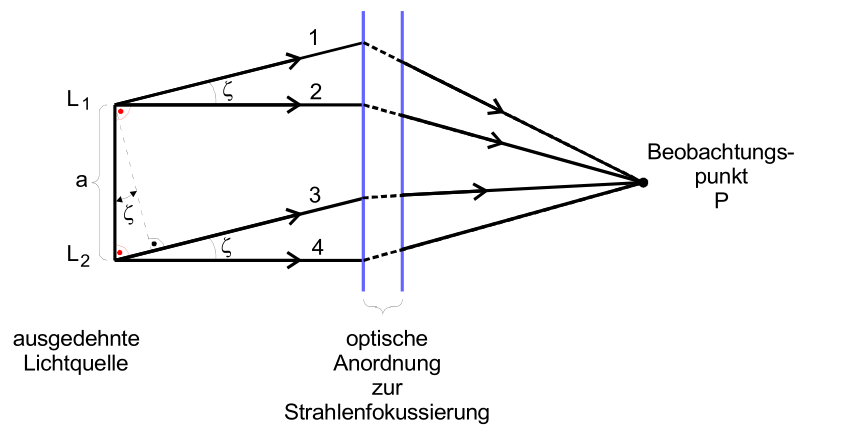
\includegraphics[width=0.3\textwidth]{build/Abb3.PNG}
    \caption {Schematischer Aufbau des Michelson-Interferometer \cite[3]{V401}.}
    \label{fig:Abb3}
\end{figure}
Im Punkt $L$ ist der Ort, wo die Lichtquelle stationiert ist, welche das Licht auf eine semipermeable Platte $P$ emittert.
Dort wird der Lichtstrahl aufgespalten, wobei ein Teil reflektiert wird und der andere transmittiert.
Beide treffen nach der Ausspaltung auf einen Spiegel, wo sie total reflektiert werden und wieder auf den semipermeablen Spiegel treffen.
Anschließend wird der beide wieder reflektiert und transmittiert. 
Zwei Strahlen treffen wieder auf den Detektor $D$. 
Damit die einzelnen Strahlen beim Wiederaufeindertreffen am semipermeablen Spiegel $P$ interferenzfähig sind, darf der Weglängenunterschied 
$ \Delta = 2\overline{\text{PS}_2} - 2\overline{\text{PS}_1} $ nicht länger als die Kohärenzlänge sein. 
Die Kompensationsplatte in der Strecke $\overline{PS_2}$ hat den gleichen Brechungsindex wie der semipermeable Spiegel; somit wird ausgeglichen,
dass der reflektierte Strahl dreimal, während der transmittierte Strahl nur einmal surch $P$ geht.\\
Sind die Strecken $\overline{PS_1}$ und $\overline{PS_2}$ gleich lang, haben die Lichtstrahlen am Detektor $D$ einen Gangunterschied von $\frac{\lambda}{2}$,
sodass destruktive Interferenz auftritt und sich die Strahlen gegenseitig auslöschen.
Wird nun einer der Spiegel um die Strecke $\Delta d$ bewegt, ändert sich das Interferenzbild und es gilt die Formel
\begin{equation}
    \Delta d = z \frac{\lambda}{2},
    \label{eqn:d}
\end{equation}
wobei $z$ die Anzahl der beobachteten Interferenzmaxima beschreibt.\\
Außerdem kann in dem Michelson-Interferometer ein optischer Weglängenunterschied aufgebut werden, in dem, wie in \autoref{fig:Abb3} zu sehen ist,
in eine der Strecken ein Medium mit einem anderen Brechungsindex eingebaut ist.
\begin{figure}[H]
    \centering
    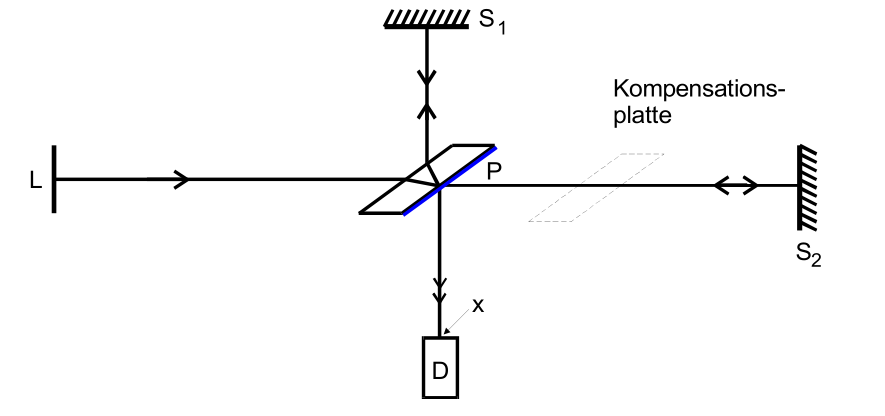
\includegraphics[width=0.3\textwidth]{build/Abb4.PNG}
    \caption {Schematischer Aufbau des Michelson-Interferometer mit Medium zur Bestimmung des Brechungsindex \cite[3]{V401}.}
    \label{fig:Abb4}
\end{figure}
Der Weglängenunterschied der beiden Strahlen beträgt $\Delta = \Delta n b$. 
Bei der Änderung vom Druck lassen sich $z$ Maxima beobachten und es gilt
\begin{equation}
    \Delta n =\frac{\lambda}{2b}.
    \label{eqn:Delta_n}
\end{equation}
Aus der klassischen Dispersionstheorie lässt sich
\begin{equation*}
    n = \sqrt{1 + f(\lambda)N}
\end{equation*}
folgern, wobei $N$ die Anzahl der Dipole pro Volumeneinheit ist, die von der Lichtwelle zu Schwingungen erwungen wurden.
Die Gase, die hier benutzt werden, verhalten sich in einem Bereich von $0$ bis $1$ bar wie ideale Gase, weswegen die ideale Gasgleichung benutzt werden kann und es gilt
\begin{equation*}
    N(r,T) = \frac{p}{T}\frac{T_0}{p_0}N_L.
\end{equation*}
Der Unterschied des Brechungsindex des Gases zu dem der Umgebung lässt sich durch $\Delta n(p,p´) = \frac{f}{2}(N(p,T)-N(p´,T))$ angeben.
Der Brechungsindex unter Normalbedingungen ergibt sich zu 
\begin{equation}
    n(p_0,T_0) = 1 + \Delta n(p,p´)\frac{T}{T_0}\frac{p_0}{p-p´},
    \label{eqn:Normalbedingungen}
\end{equation}
weswegen der Brechungsindex des Gases sich mit
\begin{equation}
    n = 1 + z \frac{\lambda}{2b} \frac{T}{T_0} \frac{p_0}{p-p´}
    \label{eqn:n}
\end{equation}
berechnen lässt.